\section{Why Layout Matters on the TPU}
\label{sec:hardware}

\subsection{The matrix unit}
\label{sec:mxu}
A TPU v3 chip has two cores, each with two MXUs; TPUGraphs timed one core, so each graph ran on two
MXUs~\cite{jouppi2020domainspecific}. Each MXU is a weight-stationary $128\times128$ grid of
multipliers that multiplies in bf16 and accumulates in fp32: a $128\times128$ block of weights sits in
the array while inputs stream through, with rows holding the reduction dimension $K$ and columns the
output channels $N$. A convolution maps to a matrix multiply with $M =$ batch $\times$ output
positions, $K = C_{\mathrm{in}} \times$ kernel height $\times$ kernel width and $N = C_{\mathrm{out}}$.
Each dimension is cut into 128-wide pieces and the last piece is zero-padded, so the useful fraction
along a dimension of size $d$ is $d / (\lceil d/128 \rceil \times 128)$ (Figure~\ref{fig:mxu}).
Section~\ref{sec:capstone} computes this utilisation for each convolution node.

\begin{figure}[t]
\centering
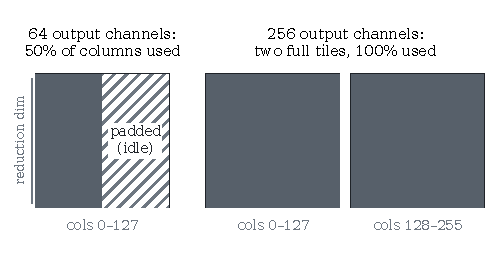
\includegraphics[width=\columnwidth]{figures/diag1_mxu_tiling.pdf}
\caption{A convolution's output channels map to the MXU's 128 columns. With 64 output channels, half
the columns sit idle as padding (left); 256 channels fill two tiles completely (right).}
\label{fig:mxu}
\end{figure}

\subsection{Tiling, roofline and contention}
\label{sec:tiling}
The compiler, not the graph, decides how each convolution is tiled onto the MXU: which dimensions to
tile and in what order, channel blocking, padding, and im2col versus direct convolution. Layout is an
input to these choices, because whether channels sit together in memory affects how they can be fed
into the array, so a layout change can change the tiling. The graph records operation types, shapes,
window sizes and layouts, but not the tiling the compiler chose. Part of a convolution's runtime
therefore depends on something no model sees (Section~\ref{sec:result2}), while the shape-based MXU
fit can still be computed from the graph (Section~\ref{sec:capstone}).

Whether MXU fit matters depends on the roofline. An operation whose arithmetic intensity (FLOPs per
byte moved) exceeds the ridge point, about 137 FLOPs/byte on TPU v3 (123 TFLOP/s $\div$ 900 GB/s), is
compute-bound, and its speed depends on how well it fills the MXU; below the ridge, memory bandwidth
dominates. Operations that need the same resource also compete for it: convolutions and dot products
share the core's two MXUs, and memory-moving operations (copy, transpose, reshape) share HBM bandwidth.
Our contention-edge model encodes this competition explicitly (Section~\ref{sec:models}).
\TODO{C11: the TPU v3 ridge $\approx$137 FLOP/byte is AI-verified only (VERIFICATION.md C11);
human-check the vendor source before submission}
